

% LaTeX path to the root directory of the current project, from the directory in which this file resides
% and path to econtexPaths which defines the rest of the paths like \FigDir
\providecommand{\econtexRoot}{}\renewcommand{\econtexRoot}{.}
\providecommand{\econtexPaths}{}\renewcommand{\econtexPaths}{\econtexRoot/Resources/econtexPaths}
% The \commands below are required to allow sharing of the same base code via Github between TeXLive on a local machine and Overleaf (which is a proxy for "a standard distribution of LaTeX").  This is an ugly solution to the requirement that custom LaTeX packages be accessible, and that Overleaf prohibits symbolic links
\providecommand{\econtex}{\econtexRoot/Resources/texmf-local/tex/latex/econtex}
\providecommand{\econtexSetup}{\econtexRoot/Resources/texmf-local/tex/latex/econtexSetup}
\providecommand{\econtexShortcuts}{\econtexRoot/Resources/texmf-local/tex/latex/econtexShortcuts}
\providecommand{\econtexBibMake}{\econtexRoot/Resources/texmf-local/tex/latex/econtexBibMake}
\providecommand{\econtexBibStyle}{\econtexRoot/Resources/texmf-local/bibtex/bst/econtex}
\providecommand{\econtexBib}{economics}
\providecommand{\notes}{\econtexRoot/Resources/texmf-local/tex/latex/handout}
\providecommand{\handoutSetup}{\econtexRoot/Resources/texmf-local/tex/latex/handoutSetup}
\providecommand{\handoutShortcuts}{\econtexRoot/Resources/texmf-local/tex/latex/handoutShortcuts}
\providecommand{\handoutBibMake}{\econtexRoot/Resources/texmf-local/tex/latex/handoutBibMake}
\providecommand{\handoutBibStyle}{\econtexRoot/Resources/texmf-local/bibtex/bst/handout}

\providecommand{\FigDir}{\econtexRoot/Figures}
\providecommand{\CodeDir}{\econtexRoot/Code}
\providecommand{\DataDir}{\econtexRoot/Data}
\providecommand{\SlideDir}{\econtexRoot/Slides}
\providecommand{\TableDir}{\econtexRoot/Tables}
\providecommand{\ApndxDir}{\econtexRoot/Appendices}

\providecommand{\ResourcesDir}{\econtexRoot/Resources}
\providecommand{\rootFromOut}{..} % Path back to root directory from output-directory
\providecommand{\LaTeXGenerated}{\econtexRoot/LaTeX} % Put generated files in subdirectory
\providecommand{\econtexPaths}{\econtexRoot/Resources/econtexPaths}
\providecommand{\LaTeXInputs}{\econtexRoot/Resources/LaTeXInputs}
\providecommand{\LtxDir}{LaTeX/}
\providecommand{\EqDir}{Equations} % Put generated files in subdirectory



\documentclass[pdflatex]{beamer}
\providecommand{\texname}{EpiExp}% Indicate the keyname for the bibtex entry corresponding to this document
\providecommand{\texnameMaster}{reference}% Indicate the keyname for the bibtex entry corresponding to this document
\newif\ifdvi\dvifalse


\usepackage{\LaTeXInputs/\texname}% Custom styles for paper

\usepackage{ifthen,dcolumn}
\provideboolean{Private}\setboolean{Private}{false}
\providecommand{\IfPrivate}{\ifthenelse{\boolean{Private}}}
\usepackage[econtex]{optional}
\usepackage{\econtexShortcuts}
\usepackage{\econtexSetup} 
\usepackage{natbib,amsmath,amssymb,rotating,subfigure}
\usepackage{verbatim,moreverb,graphicx}
\usepackage{hyperref}
\usepackage{txfonts} 
\usepackage{wasysym}
\usepackage{moreverb} 
\usepackage{comment}  
\usepackage{dcolumn}
\usepackage{cancel}
%\providecommand{\LtxDir\EqDir}{\econtexRoot/Equations}
\providecommand{\FigsRaw}{\econtexRoot/Code/Python/Figures}
\providecommand{\CodeDir}{\econtexRoot/Code}
\providecommand{\CalibrationDir}{\econtexRoot/Calibration}
\providecommand{\TableDir}{\econtexRoot/Tables}
\providecommand{\ApndxDir}{\econtexRoot/Appendices}
%\providecommand{\Ex}{\mathbb{E}}

%\usepackage{natbib}\newcommand*{\newblock}{}

\mode<presentation>
{
  \usetheme{Warsaw}
  % or ...
  \setbeamercovered{transparent}
}

%\beamerdefaultoverlayspecification{<+->}%\setbeamertemplate{navigation symbols}{}  % Take away navigation symbols

\usetheme{Warsaw}

\setbeamersize{text margin left=3mm}\setbeamersize{text margin right=3mm}

% boolean for slides
\provideboolean{Slides}
\setboolean{Slides}{true}


\title{Epidemiological Expectations in Economics}
%\subtitle{In Preparation for Handbook of Economic Expectations}
\author[Carroll, Wang]{Chris Carroll, Tao Wang}
\institute[JHU]{Johns Hopkins University}


\date{September 30, 2021}


\begin{document}
\bibliographystyle{\econtexBibStyle}

\begin{frame}[plain]
  \titlepage
\end{frame}

\section{Introduction}

\begin{frame}\frametitle{What This Paper Is Not About}
\pause
\href{https://royalsocietypublishing.org/doi/10.1098/rspa.2021.0457}{\cite{rosati2021modelling}}, Sep 24:

Epi models fit songs better than diseases:

\centerline{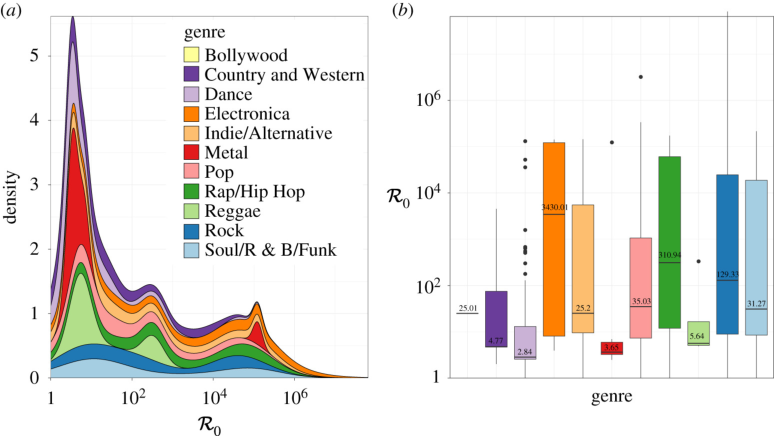
\includegraphics[width=3in]{./figures/FigureMusicR0.pdf}}

\pause $\infty$ studies: different epi models work for fads, celebrities, politics, disasters, ...
\end{frame}

\begin{frame}
    \frametitle{Why Do Economists Care About Expectations?}

    \pause Economic choices generically depend on $\mathbb{E}$

\medskip\medskip
\pause Goals:
    \begin{enumerate}
        \item Define EE: what is required to construct $\mathbb{E}$ in economic modeling
        \item Describe existing literature using EE to answer economic questions
        \begin{itemize}
            \item Technological Diffusion (entire literature)
            \item Finance (a few examples)
            \item Macroeconomics (a few examples)
        \end{itemize}
        \item Agenda for progress in building useful EE tools
    \end{enumerate}
\end{frame}

\begin{frame}
    \frametitle{Core Element of `Epidemiology'?}

Add to some existing economic model:
\pause
\begin{itemize}
    \item Social transmission of beliefs
\end{itemize}
\medskip\medskip


"Full-fledged" model requires:
  \begin{quote}\normalfont
    \begin{enumerate}
    \item \textbf{a mechanism:} \ifthenelse{\boolean{Slides}}{math by which idea(s) transmitted}{An explicit and rigorous mathematical description of a process by which ideas are communicated between agents  ...}
    \item \textbf{implying expectational dynamics:} \ifthenelse{\boolean{Slides}}{
        ... that yields observable $\mathbb{E}$ dynamics ...
      }
      {... that generates observable expectation dynamics at the level of individuals or populations~...}
    \item \textbf{with economic consequences:} \ifthenelse{\boolean{Slides}}{... those $\mathbb{E} \Rightarrow$ an economic outcome}{
        ... and those expectations have knock-on implications for an observable outcome (often, prices, quantities, or market values) that is the primary subject of the economic analysis.}
    \end{enumerate}
  \end{quote}


\medskip\medskip
\pause
\begin{itemize}
    \item ``source'' of beliefs \emph{could} be Rational
    \item if infection rate 100 percent $\rightarrow$ RE model
\end{itemize}

\end{frame}

\section{Background and Motivation}\label{motivation-and-context}

\begin{frame}
	\frametitle{Quotes}
	  \begin{quote}\ifthenelse{\boolean{Slides}}{\footnotesize}{}
    \textit{While mass media play a major role in alerting individuals to the possibility of an innovation, it seems to be personal contact that is most relevant in leading to its adoption. Thus, the diffusion of an innovation becomes a process formally akin to the spread of an infectious disease.}

    \medskip
    \indent -- %\IfPrivate{\href{https://github.com/iworld1991/EpiExp/blob/master/Literature/arrow_classificatory_1969.pdf}{\cite{arrow_classificatory_1969}}}{\cite{arrow_classificatory_1969}}
      \cite{arrow_classificatory_1969}
  \end{quote}
 %%%Slides

    \medskip

%	  \begin{quote}\ifthenelse{\boolean{Slides}}{\footnotesize}{}
    \textit{A very natural next step for economics is to maintain expectations in	the strategic position they have come to occupy, but to build an empirically validated theory of how attention is in fact directed within a social system, and how expectations are, in fact, formed.}
    \medskip
    \indent -- \href{https://econpapers.repec.org/RePEc:eee:jeborg:v:5:y:1984:i:1:p:35-55}{\cite{simon_behavioral_1984}}
  \end{quote}
 %%%Slides
%\end{frame}


%\begin{frame}
%	\frametitle{Quotes - B}
%	    \begin{quote}\ifthenelse{\boolean{Slides}}{\footnotesize}{}
      \textit{If we want to know why an unusually large economic event happened, we need to list the seemingly unrelated narratives that all happened to be going viral at around the same time and affecting the economy in the same direction.}

      % \source{
      \medskip
      \indent -- \href{https://www.amazon.com/dp/B07VZWLRM8/ref=cm_sw_em_r_mt_dp_BT5KE0VTHQX6DJ35FD9C}{\cite{shiller2017narrative}}
      % }
    \end{quote}
  
 %%%Slides
    \medskip\medskip
	  \begin{quote}\ifthenelse{\boolean{Slides}}{\footnotesize}{}
    \textit{An idea is like a virus. Resilient. Highly contagious. And even the smallest seed of an idea can grow.}   --Cobb
    \medskip \indent --
    The movie \textit{Inception} [\citeyear{Inception2010}]
  \end{quote}
 %%%Slides
\end{frame}


\subsection{Heterogeneity Matters ... }\label{EpiExpHet}\hypertarget{EpiExpHet}{}

\begin{frame}
    \frametitle{Expectational heterogeneity}
    %%%Slides
  \textit{Handbook of Microeconomics}, \href{http://larspeterhansen.org/wp-content/uploads/2016/11/Microdata-and-GE-Models.pdf}{Browning, Heckman, and Hansen [\citeyear{browning_chapter_1999}]} wrote that the most universal lesson of micro economics is that ``people are different in ways that importantly affect their economic behavior.''
%%%Slides

    \medskip\medskip

      \textit{Handbook of Macroeconomics}, \cite{kmpHandbook}: ``Macroeconomics and Household Heterogeneity'';  \cite{violante_marginal_2021} Laffont lecture on MPC Heterogeneity

  \pause \indent ~~~~~OK, heterogeneity also importantly affects ``macroeconomic'' behavior

%%%Slides

\end{frame}

\subsection{... But Is Not Yet in Models}\label{EpiExpHet}\hypertarget{EpiExpHet}{}

\begin{frame}\frametitle{Even for things like inflation or stock returns}

\begin{itemize}
    \item \cite{gmsuBeliefs}
\end{itemize}

... but not yet (regularly; as a normal practice) in ``structural'' models:

\begin{itemize}
    \item Rational Expectations
    \item Diagnostic Expectations
    \item Sparsity (Gabaix)
    \item ...
    \item Fading Memory (v 1.0)
\end{itemize}

\end{frame}

\subsection{Epidemiology REQUIRES Heterogeneity}
\begin{frame}\frametitle{Why Epidemiology?}

\begin{itemize}
    \item Other attempts (`different info sets') have not worked
    \item Vast literature outside of economics with methods, data
    \item Lots of reduced-form evidence in economics
    \item Cool new social network evidence!
\end{itemize}

\end{frame}

\subsection{Epidemiology on Networks}

\begin{frame}\frametitle{Network Theory/Graph Theory Toolkits}
    Like DYNARE for heterogeneous agent network modeling

    \begin{itemize}
        \item \texttt{NetworkX}
        \item \href{https://mybinder.org/v2/gh/llorracc/EpiExp/HEAD?filepath=SIR_Ndlib.ipynb}{NDLib}
    \end{itemize}

    These very powerful tools have been used in huge literatures outside of economics.

\end{frame}

\begin{frame}\frametitle{Two results in some tension}

    \begin{itemize}
        \item `Small World'
        \begin{itemize}
            \item 6 Degrees of Separation -- everybody is interconnected
        \end{itemize}
        \item Many ways to get persistent heterogeneity/disagreement/polarization
    \end{itemize}

\end{frame}

\subsection{Expectational Tribes}\label{subsec:ExpTribes}

\begin{frame}
		\frametitle{Expectational tribes}
\begin{figure}[!ht] \centering  % [h!]
	\caption{ ~Portfolio responses to 2016 U.S. election}
	\label{fig:parker}
	\centerline{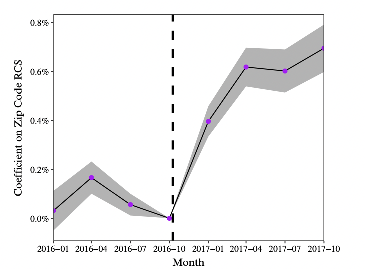
\includegraphics[width=0.6\textwidth]{./figures/parker}}
\end{figure}
\end{frame}
\section{What insights can the epidemiological framework
	offer?}\label{what-insights-can-the-epidemiological-framework-offer}



\subsection{What Is an Epidemiological Framework?}
\label{subsec: epi_framework}

\begin{frame}\frametitle{Common Source S-I Model}
  \begin{table}[ht]
    \centering
    \caption{ ~Common Source \Susceptible\Infected~Model}\label{table:SIDyn} \medskip
    \begin{tabular}{ccc}
      \hline
      Date $t$ & Susceptible$_t$ & Infected$_t$ \\
      \hline
      0 & $1$  &  $0$ \\
      \hline
      1 & $(1-p)\phantom{^2}$ & $1-(1-p)\phantom{^2}$ \\
      \hline
      2 & $(1-p)^{2}$ & $1-(1-p)^{2}$ \\
      \hline
      $\vdots$ & $\vdots$ & $\vdots$ \\
      \hline
      $n$ & $(1-p)^{n}$ & $1-(1-p)^{n}$ \\
      \hline
    \end{tabular}
  \end{table}

\end{frame}

\begin{frame}\frametitle{Personal Contact S-I Model}
      \begin{table}[ht]
    \medskip
    \caption{ ~Transmissible SI Model}\label{table:SIDynTrans}
    \centering\medskip
    \begin{tabular}{ccc}
      \hline
      Date $t$ & Susceptible$_{t}$ & Infected$_{t}$ \\
      \hline
      0 & $S_0$  &  $I_0$ \\
      \hline
      1 & $S_0 - \beta S_0I_0$ & $I_0+\beta S_0I_0$ \\
      \hline
      2 & $S_1-\beta S_1I_1$ & $I_1+\beta S_1I_1$ \\
      \hline
      $\vdots$ & $\vdots$ & $\vdots$ \\
      \hline
      $n$ & $S_{n-1}-\beta S_{n-1}I_{n-1}$ & $I_{n-1}+\beta S_{n-1}I_{n-1}$ \\
      \hline
    \end{tabular}
  \end{table}

\end{frame}

\begin{frame}\frametitle{Other States}
\begin{itemize}
    \item Recovered/Removed (Dead)
    \item Exposed (which might affect future infection risk)
    \item Immune
\end{itemize}
\end{frame}

\subsubsection{Adapting the Disease Metaphor to Expectations}\label{subsubsec:AdaptingTheModel}

\hypertarget{AdaptingTheModel}{}


\subsection{One Example}
\label{subsec:shillerpound}

\begin{frame}
	\frametitle{A SIR Model of stock investors \citep{shiller1989survey} }
	\begin{figure}[!ht] \centering  % [h!]
		\caption{ ~\href{https://mybinder.org/v2/gh/llorracc/EpiExp/HEAD?filepath=SIR_Ndlib.ipynb}{A SIR model of stock investors}}
		\label{fig:sir_diagram}
		\centerline{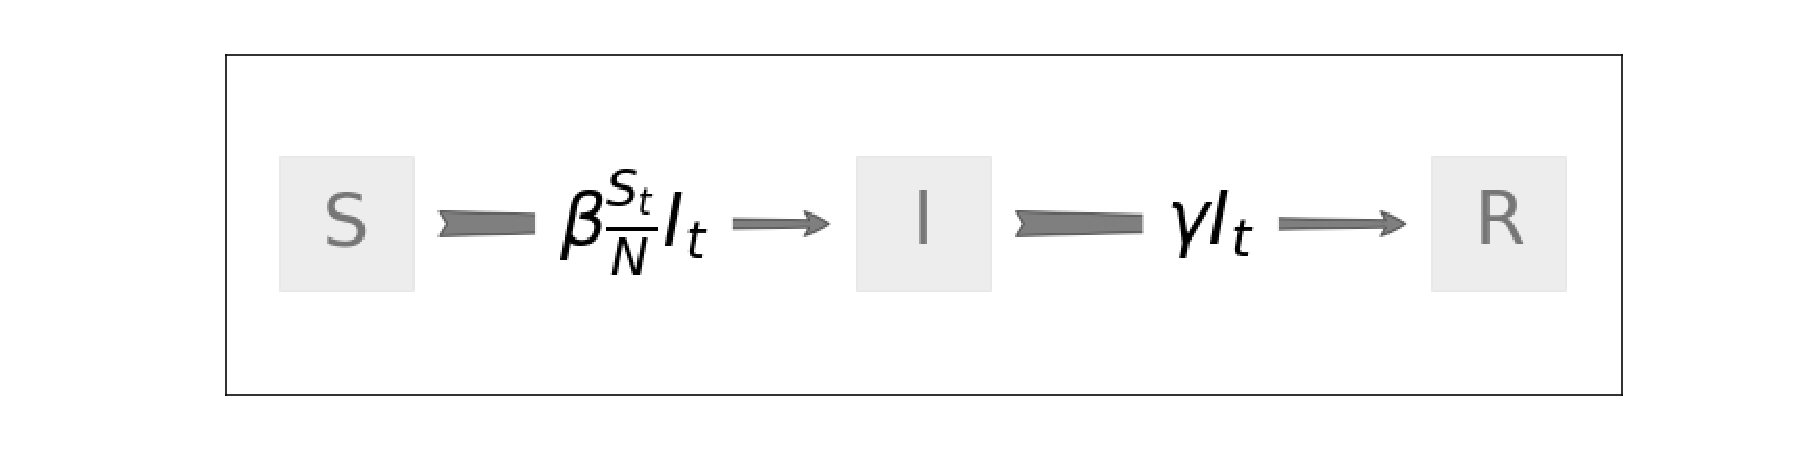
\includegraphics[width=0.7\textwidth]{./figures/flow_diagram}}
	\end{figure}
\end{frame}


\begin{frame}
		\frametitle{\href{https://mybinder.org/v2/gh/llorracc/EpiExp/HEAD?filepath=SIR_Ndlib.ipynb}{An SIR model of stock investors} }
		\begin{figure}[!ht] \centering  % [h!]
			\caption{ ~Simulated trends from an SIR model of stock investors}
			\label{fig:sir_simulate}
			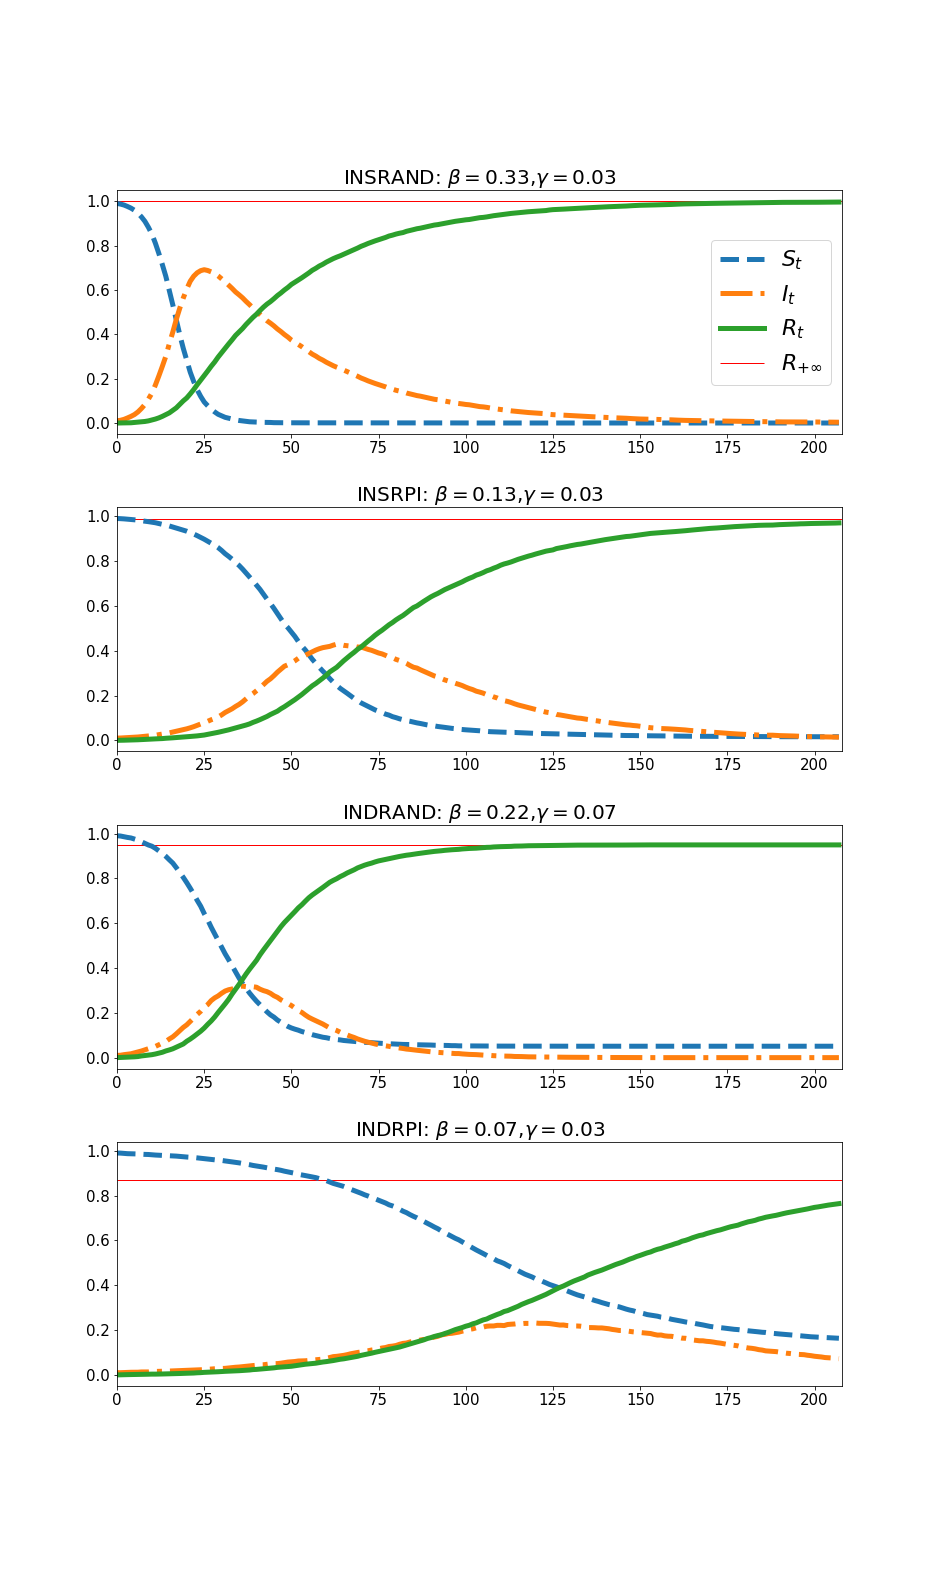
\includegraphics[width=0.85\textwidth]{./figures/sir_simulate}
		\end{figure}
\end{frame}

\section{Literature}\label{survey-of-the-literature}


\begin{frame}
	\frametitle{Three substantial fields of EE models}
%%%Slides
\begin{figure}[!ht] \centering  % [h!]
	\caption{ ~\href{https://app.litmaps.co/shared/0E6D51EB-462D-4F34-8BA2-27925D44DB8F}{Literature map}}
	\label{fig:graph_mixer}
	\centerline{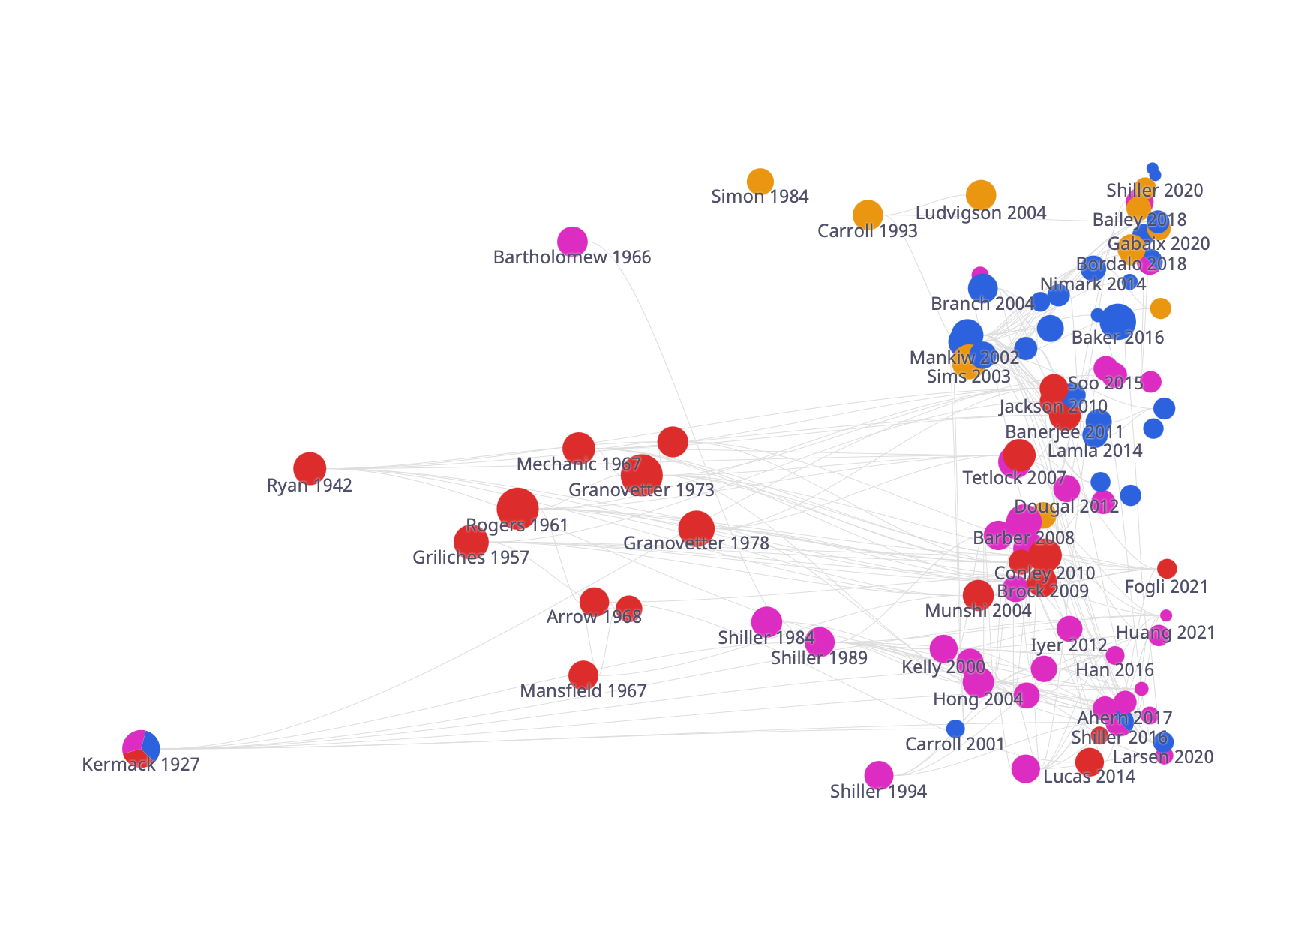
\includegraphics[width=0.65\textwidth]{./figures/graph_mixer}}
\end{figure}
\end{frame}

\subsection{Diffusion of Technology}\label{subsubsec:techDiffusion}

\begin{frame}
	\frametitle{EE models of technological diffusion}
\begin{figure}[!ht] \centering  % [h!]
	\caption{ ~\href{https://app.litmaps.co/shared/1D9003CB-75FE-4633-B60A-79B70E03B691}{Literature map of models of technological diffusion}}
	\label{fig:graph_diffusion}
	\centerline{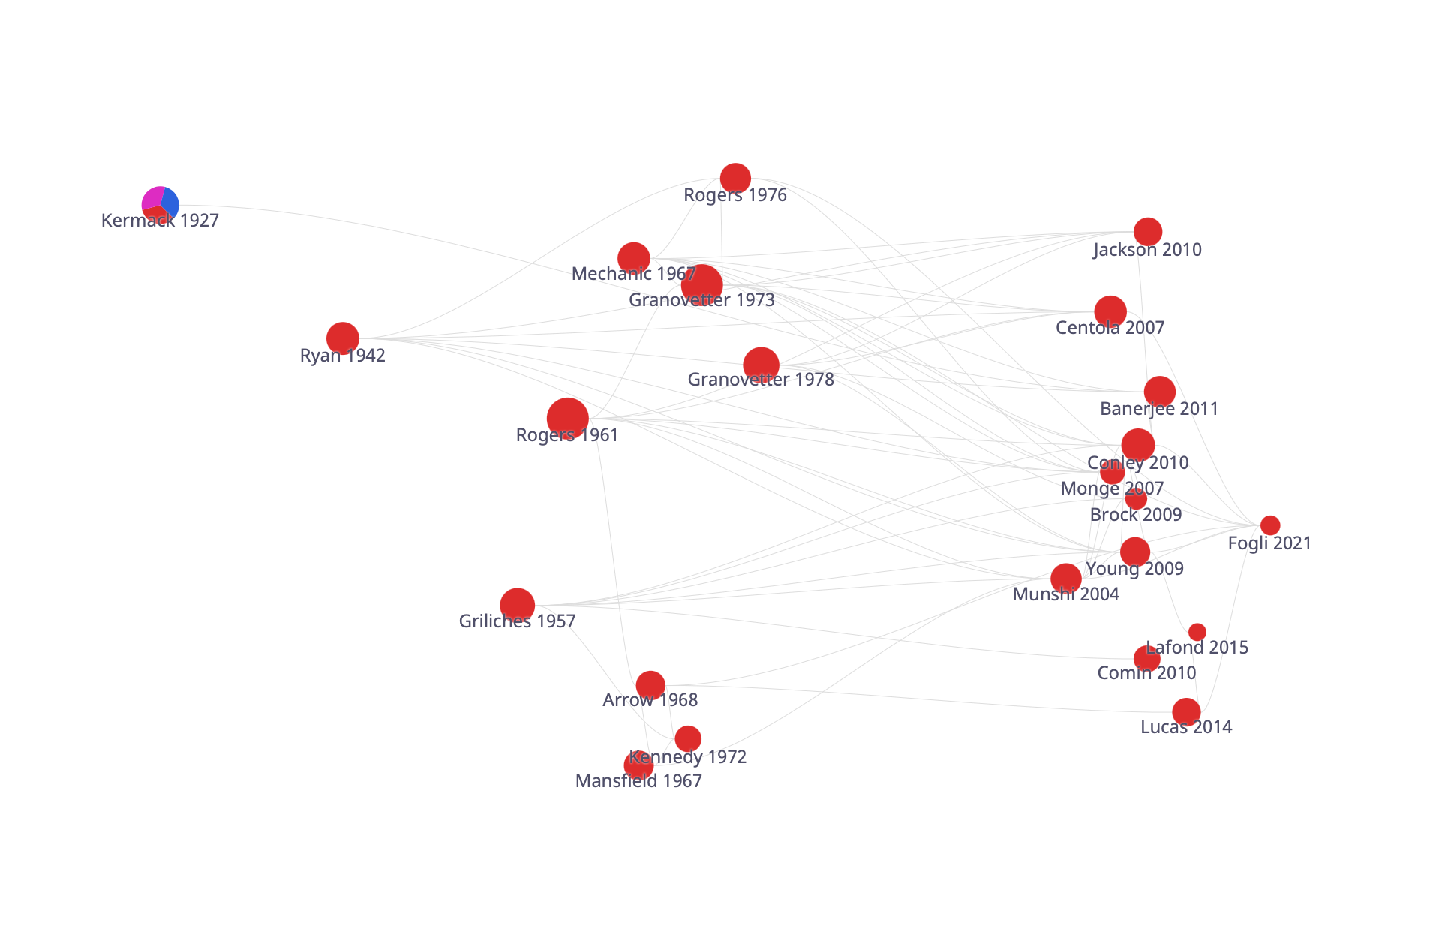
\includegraphics[width=0.65\textwidth]{./figures/graph_diffusion}}
\end{figure}
\end{frame}


\subsection{Financial Markets}\label{subsec:assetprice}

\begin{frame}
	\frametitle{EE model of asset investment}
\begin{figure}[!ht] \centering  % [h!]
	\caption{ ~\href{https://app.litmaps.co/shared/E25276CA-8725-437B-8241-11961EFB3FB4?wsid=1C4BD4E0-1E3C-4DBA-BAFD-5C50824CFC24}{Literature map of epi models of financial market investment}}
	\label{fig:graph_investment}
	\centerline{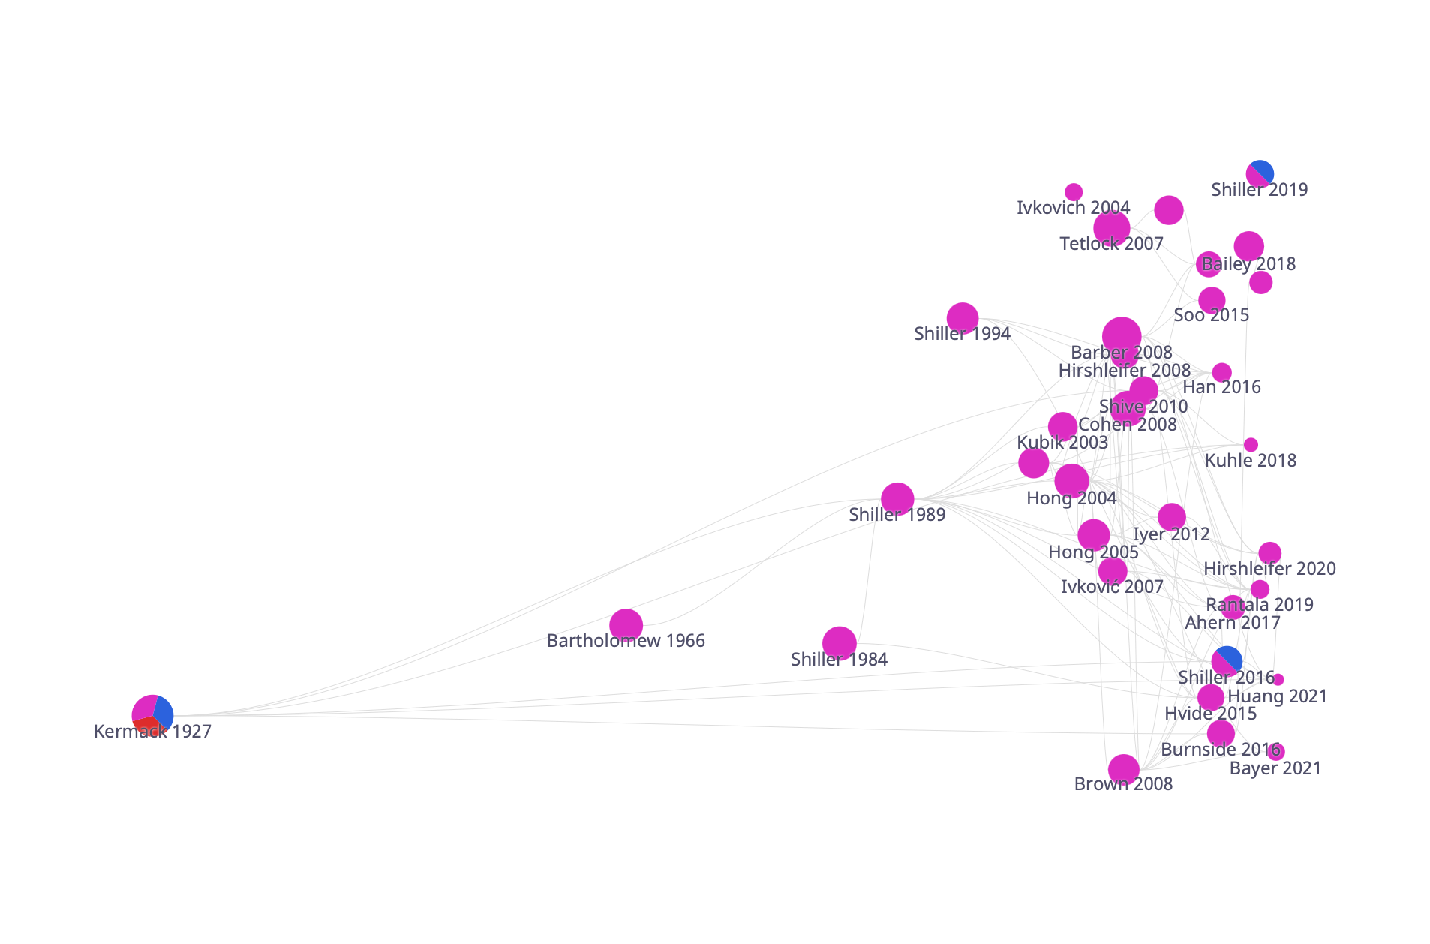
\includegraphics[width=0.65\textwidth]{./figures/graph_investment}}
\end{figure}

\end{frame}

\subsection{Macroeconomic Expectations}\label{subsec:macroExp}

\begin{frame}
	\frametitle{EE model of macroeconomic expectations}
\begin{figure}[!ht] \centering  % [h!]
	%\hypertarget{graphmacro}{}
	\caption{ ~\href{https://app.litmaps.co/shared/289F57F4-FDE5-4F94-B1A9-2BA7419DB719}{Literature map of epi models of macroeconomic expectations}}
	\label{fig:graph_macro}
	\centerline{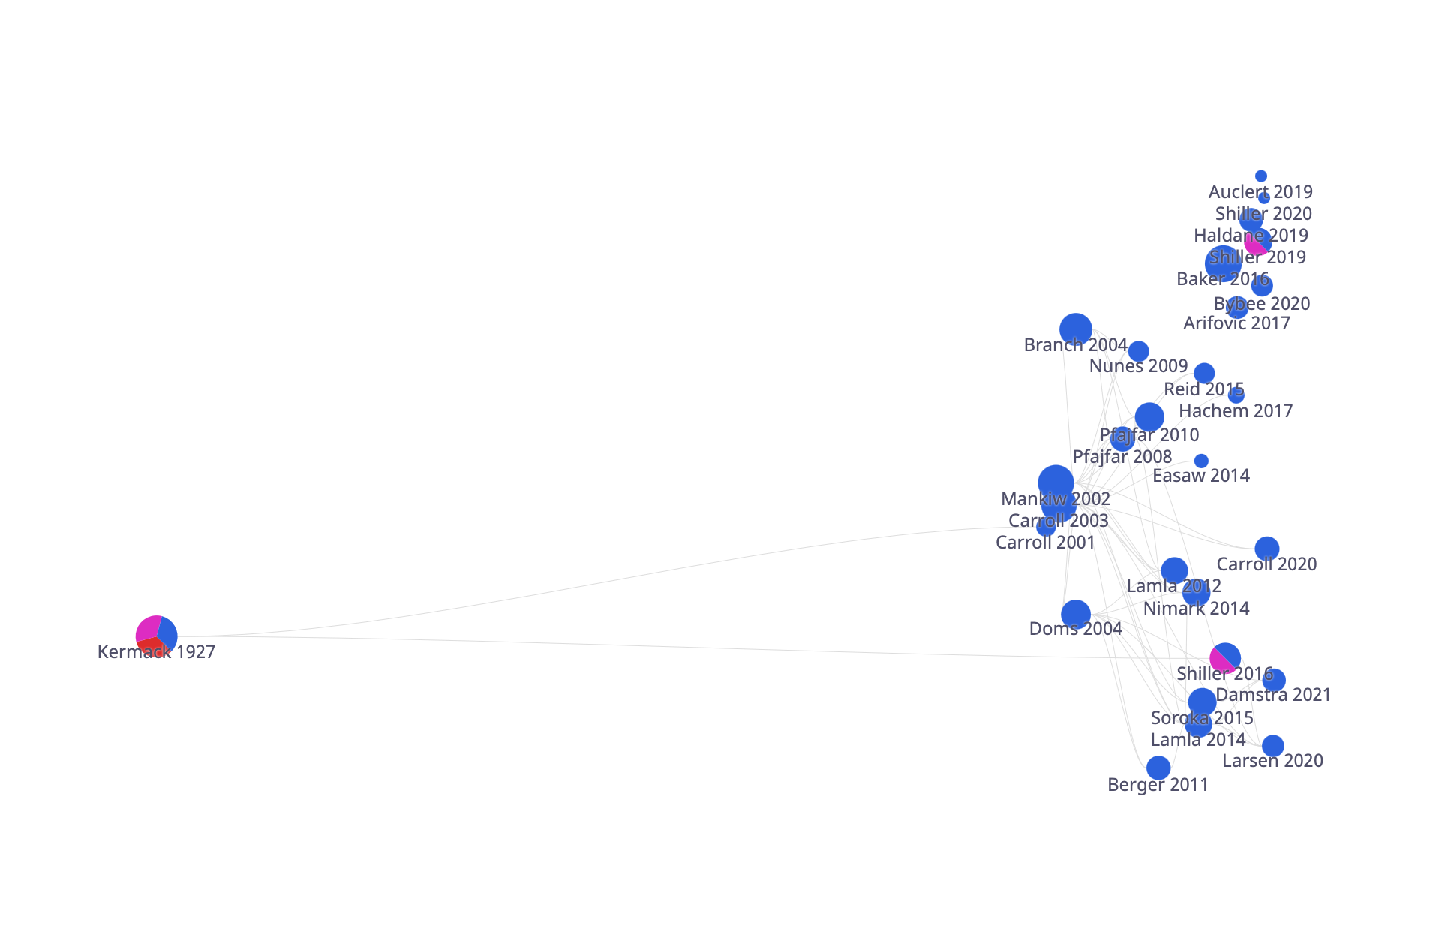
\includegraphics[width=0.65\textwidth]{./figures/graph_macro}}
\end{figure}
\end{frame}

\subsection{Contagion}\label{subsec:Contagion}

\subsection{Microeconomic Evidence}\label{subsec:microEvidence}


\begin{frame}
	\frametitle{Micro Evidence}
		  \begin{enumerate}
  \item When do socially transmitted beliefs influence important economic decisions?
  \item What are characteristics of sources and recipients of expectational infection?
  \item Through which channels are expectations mostly transmitted?
  \item What kinds of information/expectations are more infectious?
  \item How can \cite{manski1993identification}'s reflection problem be addressed?
  \end{enumerate}
 %%%Slides
\end{frame}

\subsection{Non-economic applications of epi models}
\begin{frame}
	\frametitle{Non-economic applications of epi models}
		  \begin{enumerate}
  \item the spread of news, fake news, and rumors
  \item the diffusion of scientific ideas
  \item the dissemination pattern of internet content such as memes
  \end{enumerate}
 %%%Slides
\end{frame}
\begin{frame}
	\frametitle{Other Epidemiological models}
\begin{figure}[!ht] \centering  % [h!]
	\caption{ ~\href{https://app.litmaps.co/shared/07C0B3F0-B4A9-4627-923C-857F1ABFD2D3}{Other fields related to epi models}}
	\label{fig:graph_other}
	\centerline{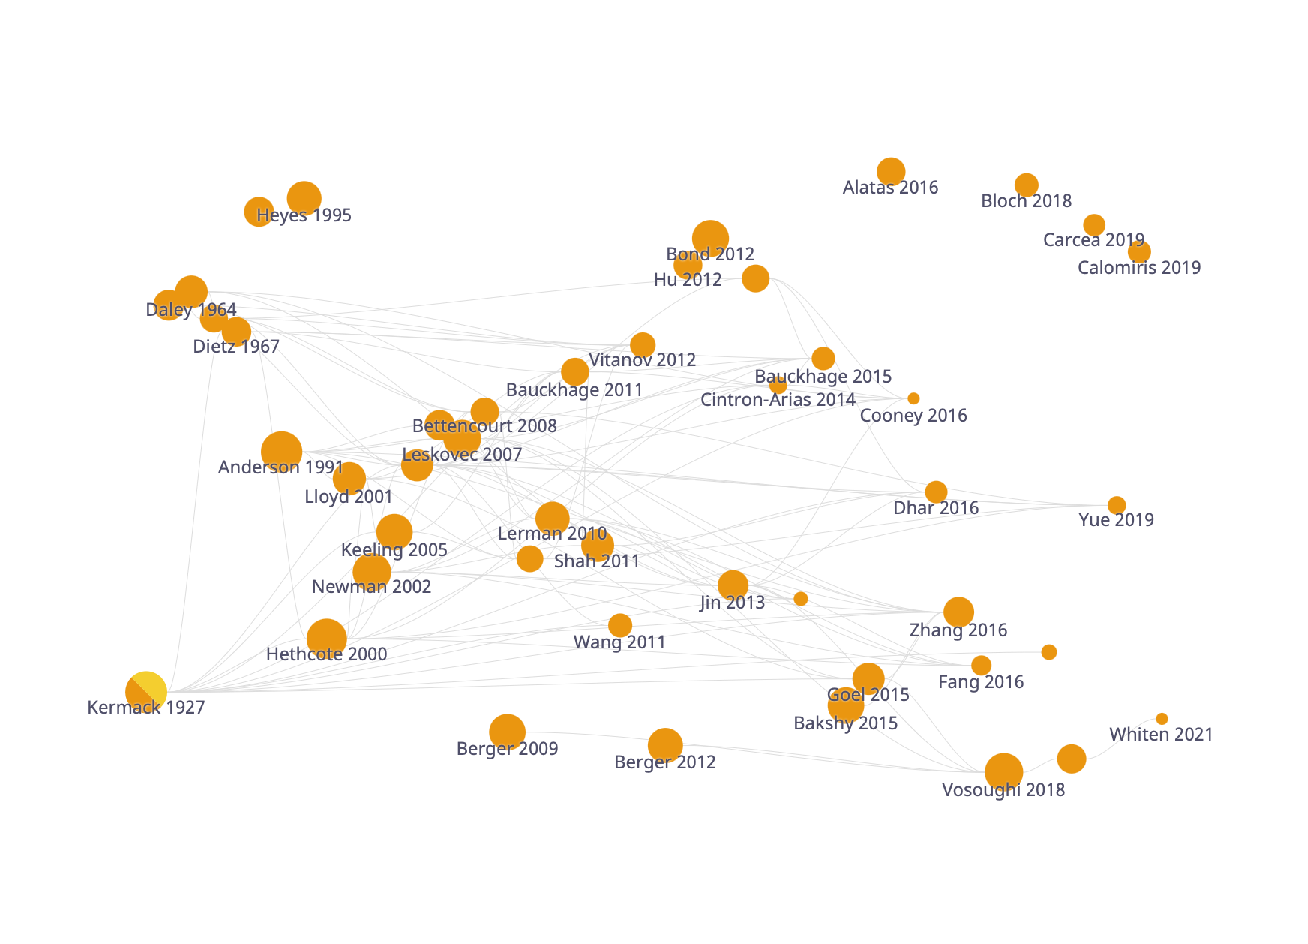
\includegraphics[width=0.65\textwidth]{./figures/graph_other}}
\end{figure}
\end{frame}


\begin{frame}
	\frametitle{An Epi model of news /rumor spreading}
\begin{figure}[!ht] \centering  % [h!]
	\caption{ ~\href{https://people.cs.vt.edu/ramakris/papers/news-rumor-epi-snakdd13.pdf}{Jin et al. (2013)}}\nocite{jin2013epidemiological}
	\label{fig:news_curve}
	\centerline{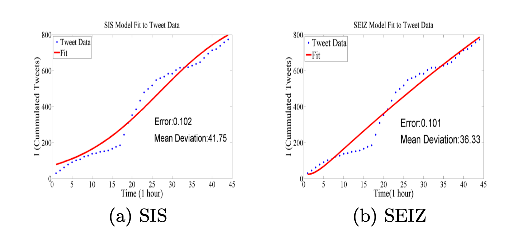
\includegraphics[width=0.7\textwidth]{./figures/Obama}}
\end{figure}
\end{frame}


\begin{frame}
	\frametitle{An Epi model of scientific ideas}
\begin{figure}[!ht] \centering  % [h!]
	\caption{ ~\href{http://web.mit.edu/dikaiser/www/BAKC.PhysA.pdf}{Bettencourt et al (2006)}}\nocite{bettencourt2006power}
	\label{fig:science_ideas_curve}
	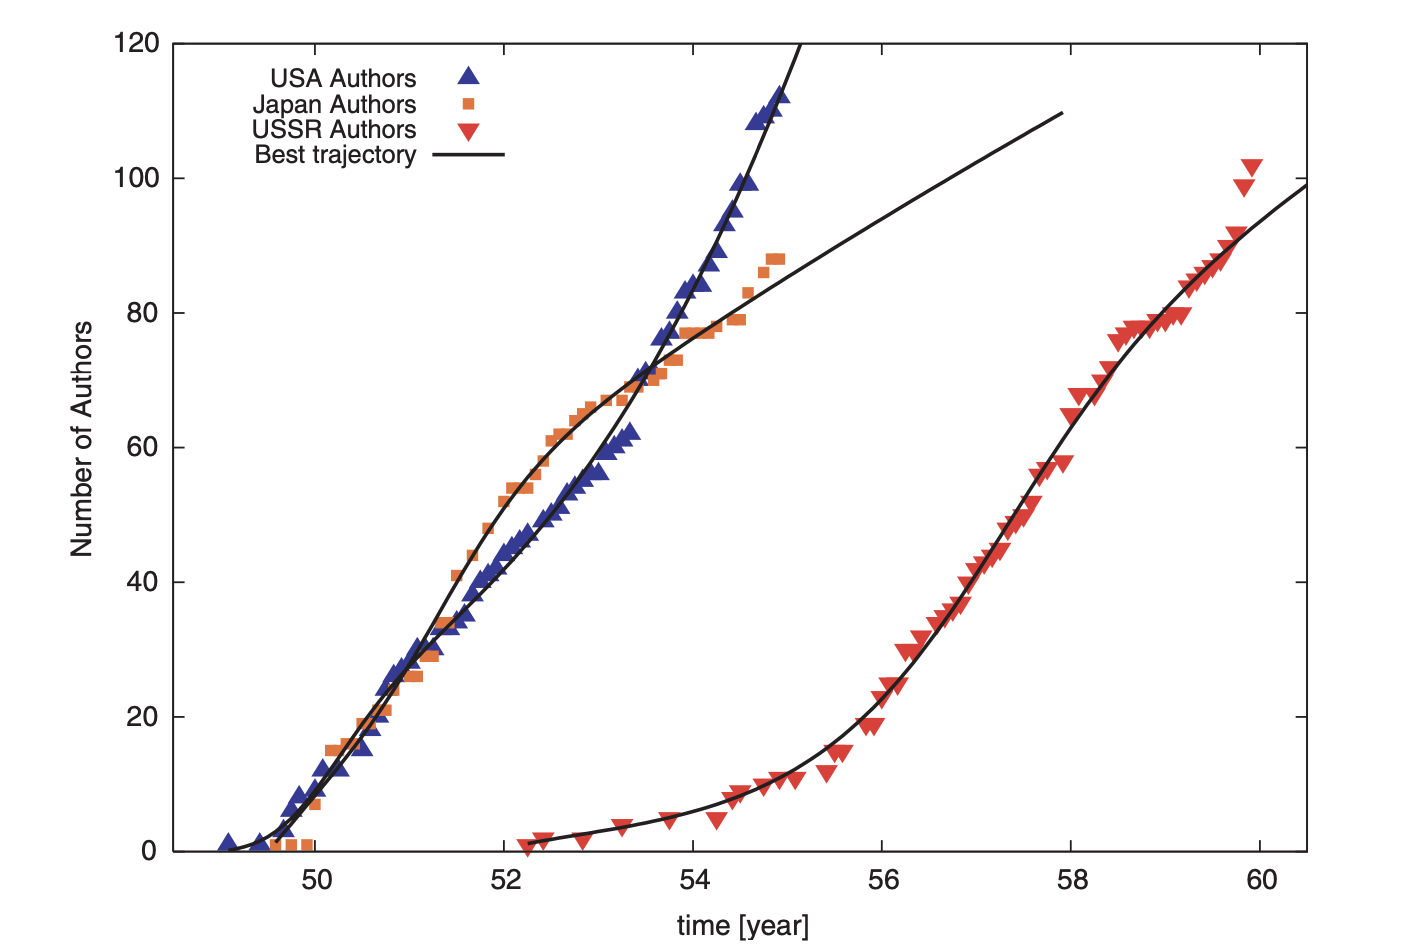
\includegraphics[width=0.7\textwidth]{./figures/Feynman}
\end{figure}
\end{frame}


\begin{frame}
	\frametitle{An Epi model of ``memes''}
	\begin{figure}[!ht] \centering  % [h!]
		\caption{ ~\href{https://github.com/iworld1991/EpiExp/blob/master/Literature/bauckhage2011insights.pdf}{\cite{bauckhage2011insights}}}
		\label{fig:memes_curve}
		\centerline{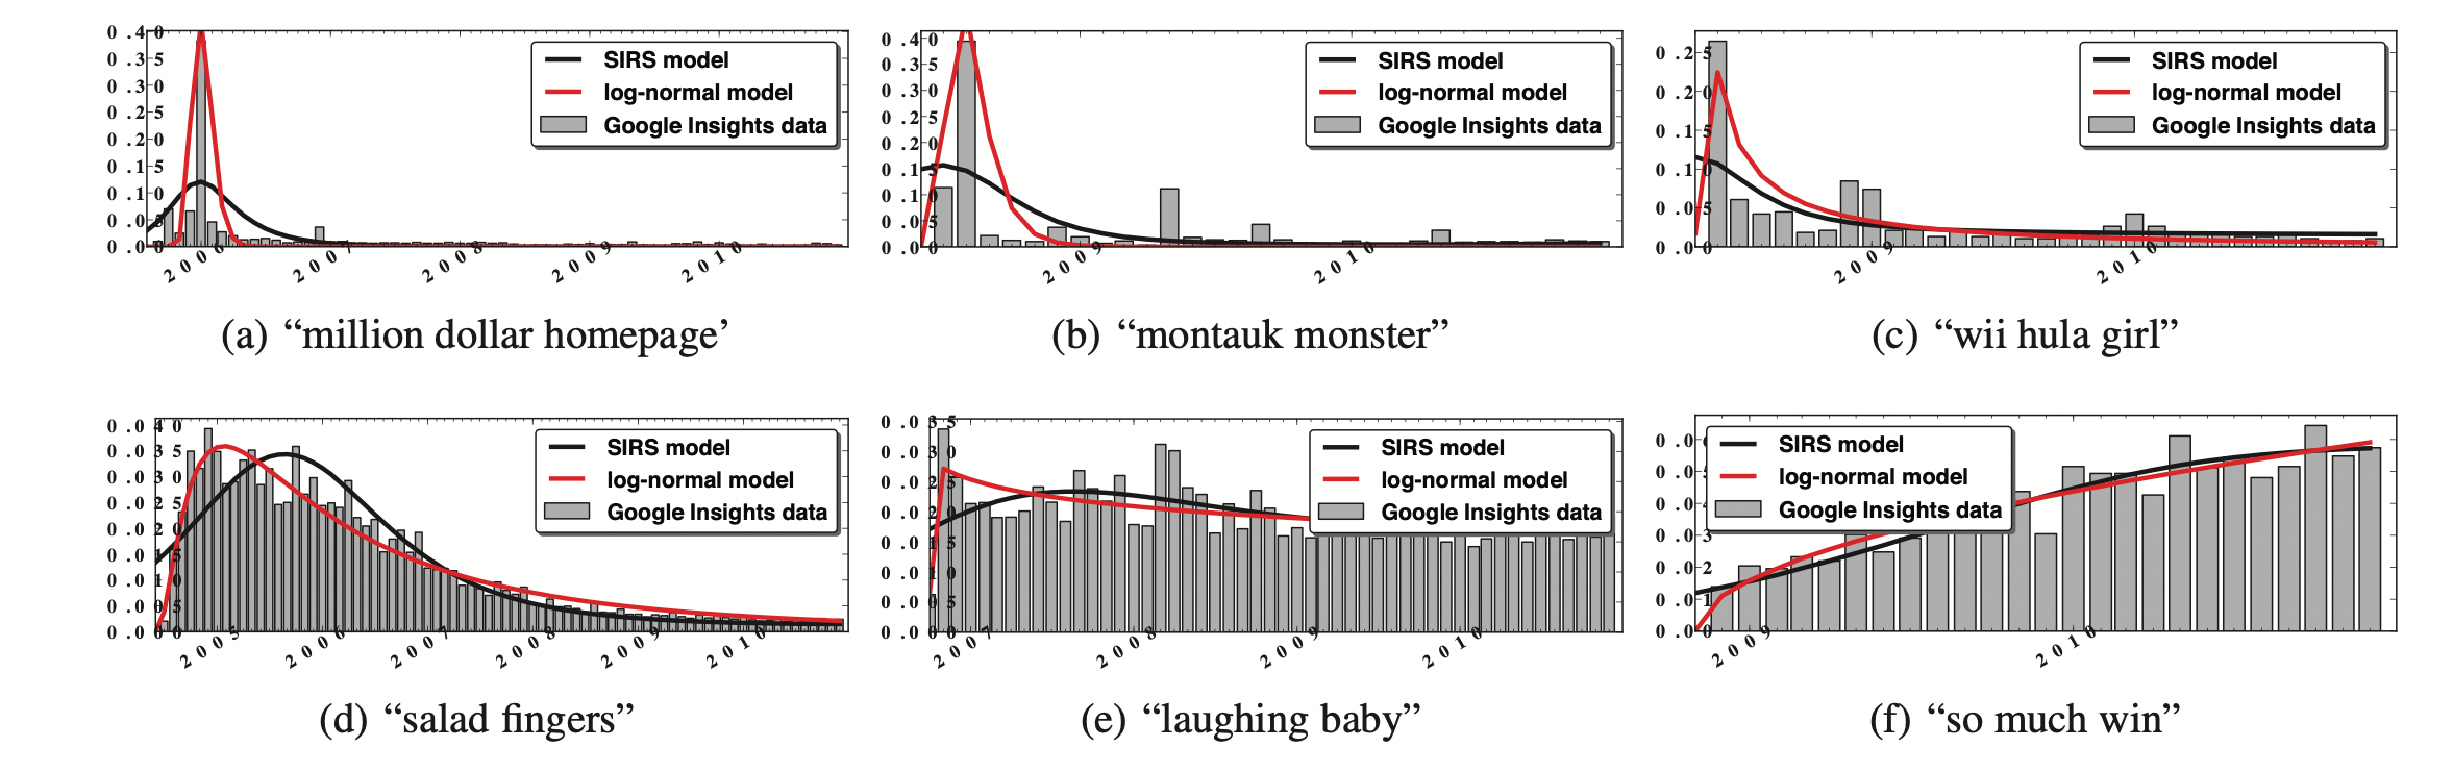
\includegraphics[width=0.7\textwidth]{./figures/Memes}}
	\end{figure}
\end{frame}


\subsection{Literature Summation}

\section{Conclusion}
\begin{frame}
	\frametitle{Conclusion}

Time is ripe for EE modeling to take off:
\begin{itemize}
    \item Data on expectations and social networks now exist!
    \item Expectations affect measured choices
    \item Mature, powerful, easy modeling \href{https://https://ndlib.readthedocs.io/en/latest/}{\texttt{NetworkX/NDLib}} tools exist
    \item HA modeling is cutting edge --
    \begin{itemize}
        \item     expectations are new frontier
    \end{itemize}
\end{itemize}

		%\input{./Slides/SlidesConclusion}
\end{frame}



\def\newblock{\hskip .11em plus .33em minus .07em}

\begin{frame}
\renewcommand{\bibsection}{\subsubsection*{\bibname }}
\tiny
\bibliography{reference}

%\bibliography{reference,\econtexBib}

\end{frame}

\end{document}\endinput

% Local Variables:
% eval: (setq TeX-command-list  (remove '("Biber" "biber %s" TeX-run-Biber nil  (plain-tex-mode latex-mode doctex-mode ams-tex-mode texinfo-mode)  :help "Run Biber") TeX-command-list))
% eval: (setq TeX-command-list  (remove '("BibTeX" "%(bibtex) %s" TeX-run-BibTeX nil t                                                                              :help "Run BibTeX") TeX-command-list))
% eval: (setq TeX-command-list  (remove '("BibTeX" "%(bibtex) %s" TeX-run-BibTeX nil (plain-tex-mode latex-mode doctex-mode ams-tex-mode texinfo-mode context-mode) :help "Run BibTeX") TeX-command-list))
% eval: (setq TeX-command-list  (remove '("BibTeX" "%(bibtex) %s" TeX-run-BibTeX nil t :help "Run BibTeX")   TeX-command-list))
% eval: (add-to-list 'TeX-command-list	'("BibTeX" "%(bibtex) %s" TeX-run-BibTeX nil t :help "Run BibTeX") t)
% eval: (cond ((string-equal system-type "darwin") (progn (setq TeX-view-program-list '(("Skim" "/Applications/Skim.app/Contents/SharedSupport/displayline -b %n %o %b"))))))
% TeX-PDF-mode: t
% TeX-file-line-error: t
% TeX-debug-warnings: t
% LaTeX-command-style: (("" "%(PDF)%(latex) %(file-line-error) %(extraopts)  %S%(PDFout)"))
% TeX-source-correlate-mode: t
% TeX-source-correlate-start-server: 0
% TeX-parse-self: t
% End:
